\section{Linear Inequalities}

\subsection{Review problems}

\begin{enumerate}
\item Solve each of the following inequalities, expressing the solution set in interval notation and graphing the solution set on a number line.
\begin{enumerate}
\item $x > -1$
\item $2x + 5\leq 7$
\item $7 - 3x < 5x - 9$
\item $(x + 4)^2 + x^2\geq (x + 2)^2 + (x + 1)^2$
\end{enumerate}
\item For each of the following combinations of inequalities, write the solution set in interval notation and graph the solution set on a number line.
\begin{enumerate}
\item $2\leq 3 + x < 6$
\item $x\geq 2 - x$ or $5 - 3x\geq x + 9$
\item $-9x + 4 < 8x + 2 < 2x + 7$
\item $-6x - 8\leq 4$ and $-x - 10\leq -7$
\item $-6x - 8\leq 4$ or $-x - 10\leq -7$
\end{enumerate}
\item \begin{enumerate}
\item Write down a pair of linear inequalities, each involving a single variable $x$, for which no real number satisfies both of the inequalities simultaneously. In this case, the solution set for ``[first inequality] and [second inequality]'' is the \emph{empty set}, denoted $\emptyset$.
\item Write down a pair of linear inequalities, each involving a single variable $x$, for which every real number satisfies at least one of the inequalities. In this case, the solution set for ``[first inequality] or [second inequality]'' is the entire set of real numbers, denoted $\mathbb{R}$. We could also write $(-\infty, \infty)$.
\item Write down a pair of linear inequalities, each involving a single variable $x$, for which the only real number which does not satisfy at least one of the inequalities is $6.626$. Express this solution set in interval notation as a union ($\cup$) of two intervals.
\end{enumerate}
\item Solve each of the following inequalities, expressing the solution set in interval notation and graphing the solution set on a number line.
\begin{enumerate}
\item $\lvert x\rvert < 4$
\item $\lvert x - 4\rvert\geq 2$
\end{enumerate}
\item Graph the solution set of each of the following inequalities.
\begin{enumerate}
\item $x + y < -2$
\item $3x - y\geq 7$
\item $(x - 1)^2 + y^2\leq (x - 5)^2 + (y - 2)^2$
\item $\lvert x\rvert + \lvert y\rvert < 1$
\end{enumerate}
\item Graph the solution set of each of the following combinations of inequalities.
\begin{enumerate}
\item $x + y\leq -2$ and $3x - y > 7$
\item $x + y < -2$ or $3x - y > 7$
\item $2x + 3y\geq 4$ and $6y\leq 12 - 4x$
\item $3x + 3y < -5x < 5y$
\end{enumerate}
\item Supposing $a\leq b$ and $c\leq d$, which of the following must also be true?
\begin{enumerate}[label=(\Roman*)]
\item $a + c\leq b + d$
\item $a - c\leq b - d$
\item $ac\leq bd$
\item $a/c\leq b/d$
\end{enumerate}
For the statements that were not guaranteed to be true, which ones are guaranteed to be true when we also assume $a\geq 0$ and $c\geq 0$?
\end{enumerate}


\subsection{Challenge problems}

\begin{enumerate}[resume]
\item Write down three inequalities for which the set of all points $(x,y)$ satisfying all of the three inequalities is the set shown below.
\begin{center}
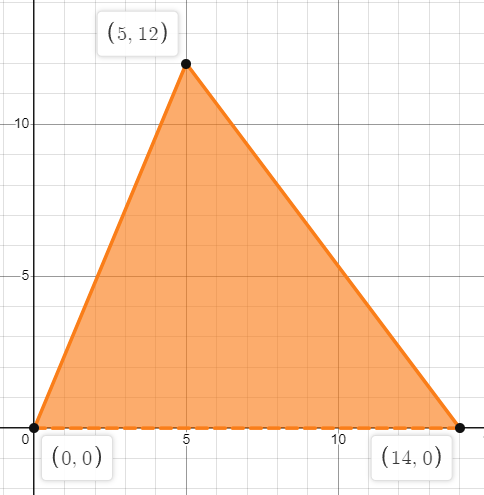
\includegraphics[scale=0.4]{lin-ineq-triangle.png}
\end{center}
\item Miko and Yuu plan to sell alms bowls and cowrie shell necklaces at their school's culture festival. Each bowl sold earns them \$30 while each necklace sold earns them \$23. Their stand will allow them to stock up to 120 items in total, and the amounts of these two items cannot differ by more than 40. (Otherwise, Miko and Yuu will start arguing so much that they drive away all potential customers.) To make the items, they need to borrow materials from the art club. Each bowl uses up 2 units of a 170-unit material allowance that the art club gives them, while each necklace uses up 1 unit of that allowance. Given all of these restrictions, what is the maximum possible amount of revenue that Miko and Yuu could bring in?
\item Find all values of $x$ for which
\begin{equation*}
\lvert\lvert x - 1\rvert - \lvert 2x - 8\rvert\rvert\leq 3/2.
\end{equation*}
Express your answer in interval notation.
\end{enumerate}


\newpage
\subsection{Answers}

In all instances of interval notation, writing $\infty$ in place of $+\infty$ would be valid (but writing $\infty$ in place of $-\infty$ would not).

\begin{enumerate}
\item \begin{enumerate}
\item $(-1, +\infty)$
\begin{center}
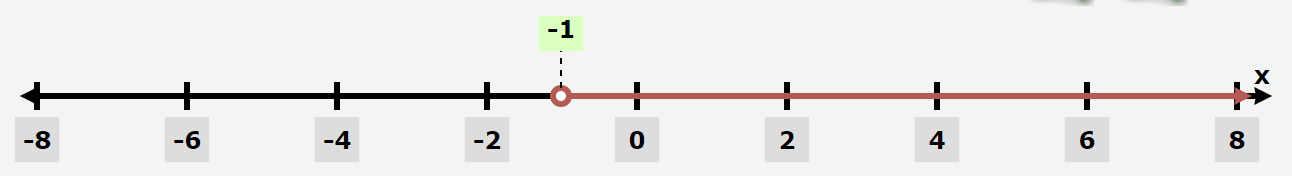
\includegraphics[scale=0.5]{lin-ineq-ans-1a.png}
\end{center}
\item $(-\infty, 1]$
\begin{center}
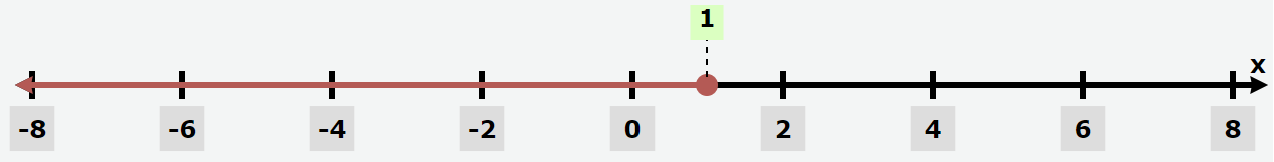
\includegraphics[scale=0.5]{lin-ineq-ans-1b.png}
\end{center}
\item $(2, +\infty)$
\begin{center}
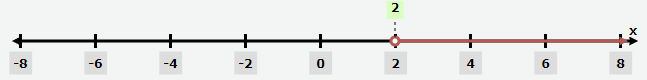
\includegraphics[scale=0.5]{lin-ineq-ans-1c.png}
\end{center}
\item $[-11/2, +\infty)$
\begin{center}
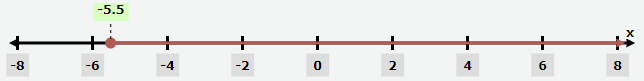
\includegraphics[scale=0.5]{lin-ineq-ans-1d.png}
\end{center}
\end{enumerate}
\item \begin{enumerate}
\item $[-1,3)$
\begin{center}
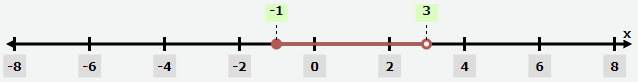
\includegraphics[scale=0.5]{lin-ineq-ans-2a.png}
\end{center}
\item $(-\infty,-1]\cup [1,+\infty)$
\begin{center}
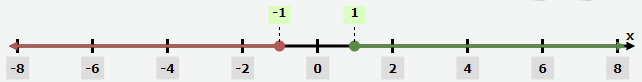
\includegraphics[scale=0.5]{lin-ineq-ans-2b.png}
\end{center}
(The colors on the graph are irrelevant.)
\item $(2/17, 5/6)$
% insert image
\item $[-2,+\infty)$
% insert image
\item $[-3,+\infty)$
% insert image
\end{enumerate}
\item There are several possible options for each of these questions.
\begin{enumerate}
\item $x > 0$ and $x < 0$
\item $x > 0$ or $x\leq 0$
\item $x > 6.626$ or $x < 6.626$
\end{enumerate}
\item The \emph{absolute value} of a real number $x$, denoted $\lvert x\rvert$, is the distance between $x$ and $0$ on the number line. A useful corollary of this is that $\lvert a - b\rvert$ is the distance between $a$ and $b$.
\begin{enumerate}
\item We want the numbers whose distance from $0$ is less than $4$, so the answer is $\boxed{(-4,4)}$.
% insert image
\item We want the numbers whose distance from $4$ is greater than or equal to $2$, so the answer is $\boxed{(-\infty,2]\cup [6, +\infty)}$.
% insert image
\end{enumerate}
\item % insert graphs, explain part d
\item % insert graphs
\item Statement (I) is the only one that is guaranteed to hold. If we introduce the additional condition that $a,c\geq 0$, so that all variables are non-negative, then statement (III) is also guaranteed to hold.
\item The bottom boundary is a dashed line segment along the $x$-axis, so to get the region above it, we can use the inequality $\boxed{y > 0}$.\par
The left boundary is a full line segment along $y = \frac{12}{5}x$, so to get a region below it, we can use the inequality $\boxed{y\leq\frac{12}{5}x}$.\par
The right boundary is a full line segment along $y = -\frac{4}{3}x + \frac{56}{3}$, so to get a region below it, we can use the inequality $\boxed{y\leq -\frac{4}{3}x + \frac{56}{3}}$.
\item Let $x$ be the number of alms bowls and $y$ be the number of cowrie shell necklaces. The problem statement imposes the following constraints on $x$ and $y$:
\begin{align*}
x &\geq 0, \\
y &\geq 0, \\
x + y &\leq 120, \tag{maximum stock} \\
x - y &\leq 40, \tag{cannot have too many more bowls} \\
y - x &\leq 40, \tag{cannot have too many more necklaces} \\
2x + y &\leq 170. \tag{materials allowance}
\end{align*}
The revenue we wish to maximise is $30x + 23y$. Our key observation for solving this type of problem (a \href{https://en.wikipedia.org/wiki/Linear_programming}{linear program}) is that a revenue $R$ can be achieved if and only if the line $30x + 23y = R$ intersects the region defined by the constraints above, so we want to find the maximum such $R$. As we increase $R$, our line moves up and to the right while retaining its slope, and when $R$ is at the desired maximum, the line will pass through a vertex of the region. (\href{https://www.desmos.com/calculator/d1towavtsb}{You can experiment with this here.}) By drawing such lines, we can identify that the vertex of interest is the intersection of the lines $x + y = 120$ and $2x + y = 170$. This intersection point is $(50,70)$, and the corresponding revenue is
\begin{equation*}
30x + 23y = 30\cdot 50 + 23\cdot 70 = \boxed{3110}.
\end{equation*}
\emph{Remark: In general, the maximum or minimum for a linear program is achieved at a vertex of the feasible region, so even without drawing lines to figure out the right vertex, we can test all of the vertices and see which one results in the largest revenue.}
\item A useful tool for handling complicated expressions involving absolute values is to consider graphs. We can interpret the given inequality as saying that we want the values of $x$ for which the vertical distance between the graphs $y = \lvert x - 1\rvert$ and $y = \lvert 2x - 8\rvert$ should be at most $3/2$. (For reference, \href{https://www.desmos.com/calculator/wowoxwrkea}{the graphs are here}.)\par 
From the graphs, we can see two intersection points whose $x$ coordinates will be part of the solution set, as the vertical distance at those values is just $0$. For the left intersection point, the lines intersecting are $y = x - 1$ and $y = -(2x - 8)$, and the intersection point is $(3,2)$. For the right intersection point, the lines intersecting are $y = x - 1$ and $y = 2x - 8$, and the intersection point is $(7,6)$.\par
As we move leftward from $(3,2)$, the blue line $y = -(2x - 8)$ moves up $2$ units for every $1$ unit left while the red line $y = x - 1$ moves down $1$ unit for every $1$ unit left, so the vertical distance between them grows by $3$ units for every $1$ unit left we move. Therefore, the graphs stay within $3/2$ of each other until we have moved $1/2$ units to the left and reached $x = 5/2$. Similarly, they stay within $3/2$ of each other as we move rightward from $(3,2)$ until we have moved $1/2$ units to the right and reached $x = 7/2$.\par
As we move from $(7,6)$, we can use similar reasoning to see that the vertical distance between the graphs grows by $1$ unit for every $1$ unit left or right we move. Thus we can move $3/2$ units left to reach $x = 11/2$ or $3/2$ units right to reach $x = 17/2$.\par 
The final answer is $\boxed{[5/2,7/2]\cup [11/2,17/2]}$.
\end{enumerate}